\documentclass[]{book}
\usepackage{lmodern}
\usepackage{amssymb,amsmath}
\usepackage{ifxetex,ifluatex}
\usepackage{fixltx2e} % provides \textsubscript
\ifnum 0\ifxetex 1\fi\ifluatex 1\fi=0 % if pdftex
  \usepackage[T1]{fontenc}
  \usepackage[utf8]{inputenc}
\else % if luatex or xelatex
  \ifxetex
    \usepackage{mathspec}
  \else
    \usepackage{fontspec}
  \fi
  \defaultfontfeatures{Ligatures=TeX,Scale=MatchLowercase}
\fi
% use upquote if available, for straight quotes in verbatim environments
\IfFileExists{upquote.sty}{\usepackage{upquote}}{}
% use microtype if available
\IfFileExists{microtype.sty}{%
\usepackage{microtype}
\UseMicrotypeSet[protrusion]{basicmath} % disable protrusion for tt fonts
}{}
\usepackage[margin=1in]{geometry}
\usepackage{hyperref}
\hypersetup{unicode=true,
            pdftitle={Time Series and Longitudinal Analysis},
            pdfauthor={Richard White},
            pdfborder={0 0 0},
            breaklinks=true}
\urlstyle{same}  % don't use monospace font for urls
\usepackage{natbib}
\bibliographystyle{apalike}
\usepackage{color}
\usepackage{fancyvrb}
\newcommand{\VerbBar}{|}
\newcommand{\VERB}{\Verb[commandchars=\\\{\}]}
\DefineVerbatimEnvironment{Highlighting}{Verbatim}{commandchars=\\\{\}}
% Add ',fontsize=\small' for more characters per line
\usepackage{framed}
\definecolor{shadecolor}{RGB}{248,248,248}
\newenvironment{Shaded}{\begin{snugshade}}{\end{snugshade}}
\newcommand{\KeywordTok}[1]{\textcolor[rgb]{0.13,0.29,0.53}{\textbf{#1}}}
\newcommand{\DataTypeTok}[1]{\textcolor[rgb]{0.13,0.29,0.53}{#1}}
\newcommand{\DecValTok}[1]{\textcolor[rgb]{0.00,0.00,0.81}{#1}}
\newcommand{\BaseNTok}[1]{\textcolor[rgb]{0.00,0.00,0.81}{#1}}
\newcommand{\FloatTok}[1]{\textcolor[rgb]{0.00,0.00,0.81}{#1}}
\newcommand{\ConstantTok}[1]{\textcolor[rgb]{0.00,0.00,0.00}{#1}}
\newcommand{\CharTok}[1]{\textcolor[rgb]{0.31,0.60,0.02}{#1}}
\newcommand{\SpecialCharTok}[1]{\textcolor[rgb]{0.00,0.00,0.00}{#1}}
\newcommand{\StringTok}[1]{\textcolor[rgb]{0.31,0.60,0.02}{#1}}
\newcommand{\VerbatimStringTok}[1]{\textcolor[rgb]{0.31,0.60,0.02}{#1}}
\newcommand{\SpecialStringTok}[1]{\textcolor[rgb]{0.31,0.60,0.02}{#1}}
\newcommand{\ImportTok}[1]{#1}
\newcommand{\CommentTok}[1]{\textcolor[rgb]{0.56,0.35,0.01}{\textit{#1}}}
\newcommand{\DocumentationTok}[1]{\textcolor[rgb]{0.56,0.35,0.01}{\textbf{\textit{#1}}}}
\newcommand{\AnnotationTok}[1]{\textcolor[rgb]{0.56,0.35,0.01}{\textbf{\textit{#1}}}}
\newcommand{\CommentVarTok}[1]{\textcolor[rgb]{0.56,0.35,0.01}{\textbf{\textit{#1}}}}
\newcommand{\OtherTok}[1]{\textcolor[rgb]{0.56,0.35,0.01}{#1}}
\newcommand{\FunctionTok}[1]{\textcolor[rgb]{0.00,0.00,0.00}{#1}}
\newcommand{\VariableTok}[1]{\textcolor[rgb]{0.00,0.00,0.00}{#1}}
\newcommand{\ControlFlowTok}[1]{\textcolor[rgb]{0.13,0.29,0.53}{\textbf{#1}}}
\newcommand{\OperatorTok}[1]{\textcolor[rgb]{0.81,0.36,0.00}{\textbf{#1}}}
\newcommand{\BuiltInTok}[1]{#1}
\newcommand{\ExtensionTok}[1]{#1}
\newcommand{\PreprocessorTok}[1]{\textcolor[rgb]{0.56,0.35,0.01}{\textit{#1}}}
\newcommand{\AttributeTok}[1]{\textcolor[rgb]{0.77,0.63,0.00}{#1}}
\newcommand{\RegionMarkerTok}[1]{#1}
\newcommand{\InformationTok}[1]{\textcolor[rgb]{0.56,0.35,0.01}{\textbf{\textit{#1}}}}
\newcommand{\WarningTok}[1]{\textcolor[rgb]{0.56,0.35,0.01}{\textbf{\textit{#1}}}}
\newcommand{\AlertTok}[1]{\textcolor[rgb]{0.94,0.16,0.16}{#1}}
\newcommand{\ErrorTok}[1]{\textcolor[rgb]{0.64,0.00,0.00}{\textbf{#1}}}
\newcommand{\NormalTok}[1]{#1}
\usepackage{longtable,booktabs}
\usepackage{graphicx,grffile}
\makeatletter
\def\maxwidth{\ifdim\Gin@nat@width>\linewidth\linewidth\else\Gin@nat@width\fi}
\def\maxheight{\ifdim\Gin@nat@height>\textheight\textheight\else\Gin@nat@height\fi}
\makeatother
% Scale images if necessary, so that they will not overflow the page
% margins by default, and it is still possible to overwrite the defaults
% using explicit options in \includegraphics[width, height, ...]{}
\setkeys{Gin}{width=\maxwidth,height=\maxheight,keepaspectratio}
\IfFileExists{parskip.sty}{%
\usepackage{parskip}
}{% else
\setlength{\parindent}{0pt}
\setlength{\parskip}{6pt plus 2pt minus 1pt}
}
\setlength{\emergencystretch}{3em}  % prevent overfull lines
\providecommand{\tightlist}{%
  \setlength{\itemsep}{0pt}\setlength{\parskip}{0pt}}
\setcounter{secnumdepth}{5}
% Redefines (sub)paragraphs to behave more like sections
\ifx\paragraph\undefined\else
\let\oldparagraph\paragraph
\renewcommand{\paragraph}[1]{\oldparagraph{#1}\mbox{}}
\fi
\ifx\subparagraph\undefined\else
\let\oldsubparagraph\subparagraph
\renewcommand{\subparagraph}[1]{\oldsubparagraph{#1}\mbox{}}
\fi

%%% Use protect on footnotes to avoid problems with footnotes in titles
\let\rmarkdownfootnote\footnote%
\def\footnote{\protect\rmarkdownfootnote}

%%% Change title format to be more compact
\usepackage{titling}

% Create subtitle command for use in maketitle
\newcommand{\subtitle}[1]{
  \posttitle{
    \begin{center}\large#1\end{center}
    }
}

\setlength{\droptitle}{-2em}

  \title{Time Series and Longitudinal Analysis}
    \pretitle{\vspace{\droptitle}\centering\huge}
  \posttitle{\par}
    \author{Richard White}
    \preauthor{\centering\large\emph}
  \postauthor{\par}
      \predate{\centering\large\emph}
  \postdate{\par}
    \date{2018-11-02}

\usepackage{booktabs}

\begin{document}
\maketitle

{
\setcounter{tocdepth}{1}
\tableofcontents
}
\chapter*{Preface}\label{preface}
\addcontentsline{toc}{chapter}{Preface}

When dealing with data measured over time, there are two kinds of
analyses that can be performed.

``Time series'' analyses generally deal with one variable (the outcome).
We can then either:

\begin{enumerate}
\def\labelenumi{\arabic{enumi}.}
\tightlist
\item
  Predict the future only using the previous observations. E.g. predict
  tomorrow's temperature, using today's and yesterday's temperature as
  exposures. We will not be focusing on these kinds of analyses.
\item
  Estimate descriptive statistics about the data. E.g. Today's data is
  much higher than expected (outbreak?). We will focus on these kinds of
  analyses.
\end{enumerate}

If we have more than one variable measured over time (e.g.~outcome and
an exposure) then we can run regression analyses. E.g. seeing how the
number of tuberculosis patients (outcome) is affected by the number of
immigrants to Norway (exposure) over a 20 year period. We will focus on
these kinds of analyses.

It is important to note that if we define our exposure as ``time'' then
we can use the regression framework to estimate descriptive statistics
about the data. This means we can use the same regression framework for
the two kinds of analyses we will be focusing on.

``Regression analyses'' are very similar to ordinary regressions that
you have been working with for many years. The only difference is that
they \textbf{may} have more advanced data structures that your normal
methods cannot handle.

\chapter{Reference}\label{reference}

\section{Scope of this course}\label{scope-of-this-course}

When dealing with longitudinal data, there are two kinds of analyses
that can be performed.

``Time series'' analyses generally deal with one variable. The aim is to
then predict the future only using the previous observations. A common
example would be to predict tomorrow's temperature, using today's and
yesterday's temperature as exposures. We will not be focusing on these
kinds of analyses.

``Regression analyses'' are very similar to ordinary regressions that
you have been working with for many years. The only difference is that
they \textbf{may} have more advanced data structures that your current
methods cannot handle.

For example, if you want to see how the number of tuberculosis patients
(outcome) is affected by the number of immigrants to Norway (exposure)
over a 20 year period, then the number of patients in each year might be
associated with each other, which might break assumptions of the
regression models that you normally use (independent residuals). To
account for the advanced structure of the data (correlation between
different years) we will use more advanced regression techniques. This
is what we will be focusing on in this course.

To recap: this course will let you run ``normal regressions'' in
situations where the data structure would ordinarily prohibit you from
running regression models. These situations mostly pertain to clusters
of correlated data.

\newpage

\section{Introduction}\label{introduction}

There are two important definitions in this course:

\begin{itemize}
\tightlist
\item
  Panel data
\item
  Autocorrelation
\end{itemize}

Panel data is a set of data with measurements repeated at equally spaced
points. For example, weight data recorded every day, or every week, or
every year would be considered panel data. A person who records three
weight measurements randomly in 2018 would not be considered panel data.

When you have panel data, autocorrelation is the correlation between
subsequent observations. For example, if you have daily observations,
then the 1 day autocorrelation is the correlation between observations 1
day apart, and likewise the 2 day autocorrelation is the correlation
between observations 2 days apart.

In this course we will consider 5 scenarios where we have multiple
observations for each geographical area:

\begin{itemize}
\tightlist
\item
  Panel data: One geographical area, no autocorrelation
\item
  Panel data: One geographical area, with autocorrelation
\item
  Not panel data: Multiple geographical areas
\item
  Panel data: Multiple geographical areas, no autocorrelation
\item
  Panel data: Multiple geographical areas, with autocorrelation
\end{itemize}

Note, the following scenario can be covered by standard regression
models:

\begin{itemize}
\tightlist
\item
  Multiple geographical areas, one time point/observation per
  geographical area
\end{itemize}

\newpage

\section{Method summary}\label{method-summary}

\subsection{Panel data: One geographical area, no
autocorrelation}\label{panel-data-one-geographical-area-no-autocorrelation}

\begin{verbatim}
// STATA CODE
glm y yearminus2000 dailyrainfall cos365 sin365, family(poisson)
\end{verbatim}

\begin{Shaded}
\begin{Highlighting}[]
\CommentTok{# R CODE}
\NormalTok{fit1 <-}\StringTok{ }\KeywordTok{glm}\NormalTok{(y}\OperatorTok{~}\NormalTok{yearMinus2000 }\OperatorTok{+}\StringTok{ }\NormalTok{dailyrainfall }\OperatorTok{+}\StringTok{ }\NormalTok{sin365 }\OperatorTok{+}\StringTok{ }\NormalTok{cos365, }\DataTypeTok{data=}\NormalTok{d, }\DataTypeTok{family=}\KeywordTok{poisson}\NormalTok{())}
\KeywordTok{residuals}\NormalTok{(fit1, }\DataTypeTok{type =} \StringTok{"response"}\NormalTok{)}
\end{Highlighting}
\end{Shaded}

\subsection{Panel data: One geographical area, with
autocorrelation}\label{panel-data-one-geographical-area-with-autocorrelation}

\begin{verbatim}
// STATA CODE
glm y yearminus2000 cos365 sin365, family(poisson) vce(robust)
\end{verbatim}

\begin{Shaded}
\begin{Highlighting}[]
\CommentTok{# R CODE}
\NormalTok{fit <-}\StringTok{ }\NormalTok{MASS}\OperatorTok{::}\KeywordTok{glmmPQL}\NormalTok{(y}\OperatorTok{~}\NormalTok{yearMinus2000}\OperatorTok{+}\NormalTok{sin365 }\OperatorTok{+}\StringTok{ }\NormalTok{cos365, }\DataTypeTok{random =} \OperatorTok{~}\StringTok{ }\DecValTok{1} \OperatorTok{|}\StringTok{ }\NormalTok{ID,}
                \DataTypeTok{family =}\NormalTok{ poisson, }\DataTypeTok{data =}\NormalTok{ d,}
                \DataTypeTok{correlation=}\NormalTok{nlme}\OperatorTok{::}\KeywordTok{corAR1}\NormalTok{(}\DataTypeTok{form=}\OperatorTok{~}\NormalTok{dayOfSeries}\OperatorTok{|}\NormalTok{ID))}
\NormalTok{r <-}\StringTok{ }\KeywordTok{residuals}\NormalTok{(fit1, }\DataTypeTok{type =} \StringTok{"normalized"}\NormalTok{)}
\KeywordTok{pacf}\NormalTok{(r)}
\end{Highlighting}
\end{Shaded}

\subsection{Not panel data: Multiple geographical
areas}\label{not-panel-data-multiple-geographical-areas}

\begin{verbatim}
// STATA CODE
meglm y x yearMinus2000 || fylke:, family(poisson)
\end{verbatim}

\begin{Shaded}
\begin{Highlighting}[]
\CommentTok{# R CODE}
\NormalTok{fit <-}\StringTok{ }\NormalTok{lme4}\OperatorTok{::}\KeywordTok{glmer}\NormalTok{(y}\OperatorTok{~}\NormalTok{x }\OperatorTok{+}\StringTok{ }\NormalTok{yearMinus2000 }\OperatorTok{+}\StringTok{ }\NormalTok{(}\DecValTok{1}\OperatorTok{|}\NormalTok{fylke),}\DataTypeTok{data=}\NormalTok{d,}\DataTypeTok{family=}\KeywordTok{poisson}\NormalTok{())}
\end{Highlighting}
\end{Shaded}

\subsection{Panel data: Multiple geographical areas, no
autocorrelation}\label{panel-data-multiple-geographical-areas-no-autocorrelation}

\begin{verbatim}
// STATA CODE
meglm y yearminus2000 cos365 sin365 || fylke:, family(poisson)
\end{verbatim}

\begin{Shaded}
\begin{Highlighting}[]
\CommentTok{# R CODE}
\NormalTok{fit <-}\StringTok{ }\NormalTok{MASS}\OperatorTok{::}\KeywordTok{glmmPQL}\NormalTok{(y}\OperatorTok{~}\NormalTok{yearMinus2000}\OperatorTok{+}\NormalTok{sin365 }\OperatorTok{+}\StringTok{ }\NormalTok{cos365, }\DataTypeTok{random =} \OperatorTok{~}\StringTok{ }\DecValTok{1} \OperatorTok{|}\StringTok{ }\NormalTok{fylke,}
                \DataTypeTok{family =}\NormalTok{ poisson, }\DataTypeTok{data =}\NormalTok{ d)}
\NormalTok{r <-}\StringTok{ }\KeywordTok{residuals}\NormalTok{(fit1, }\DataTypeTok{type =} \StringTok{"normalized"}\NormalTok{)}
\KeywordTok{pacf}\NormalTok{(r)}
\end{Highlighting}
\end{Shaded}

\subsection{Panel data: Multiple geographical areas, with
autocorrelation}\label{panel-data-multiple-geographical-areas-with-autocorrelation}

\begin{verbatim}
// STATA CODE
meglm y yearminus2000 cos365 sin365 || fylke:, family(poisson) vce(robust)
\end{verbatim}

\begin{Shaded}
\begin{Highlighting}[]
\CommentTok{# R CODE}
\NormalTok{fit <-}\StringTok{ }\NormalTok{MASS}\OperatorTok{::}\KeywordTok{glmmPQL}\NormalTok{(y}\OperatorTok{~}\NormalTok{yearMinus2000}\OperatorTok{+}\NormalTok{sin365 }\OperatorTok{+}\StringTok{ }\NormalTok{cos365, }\DataTypeTok{random =} \OperatorTok{~}\StringTok{ }\DecValTok{1} \OperatorTok{|}\StringTok{ }\NormalTok{fylke,}
                \DataTypeTok{family =}\NormalTok{ poisson, }\DataTypeTok{data =}\NormalTok{ d,}
                \DataTypeTok{correlation=}\NormalTok{nlme}\OperatorTok{::}\KeywordTok{corAR1}\NormalTok{(}\DataTypeTok{form=}\OperatorTok{~}\NormalTok{dayOfSeries}\OperatorTok{|}\NormalTok{fylke))}
\NormalTok{r <-}\StringTok{ }\KeywordTok{residuals}\NormalTok{(fit1, }\DataTypeTok{type =} \StringTok{"normalized"}\NormalTok{)}
\KeywordTok{pacf}\NormalTok{(r)}
\end{Highlighting}
\end{Shaded}

\newpage

\section{Identifying your scenario}\label{identifying-your-scenario}

\subsection{Step 1: Do you have panel
data?}\label{step-1-do-you-have-panel-data}

This step should be fairly simple. If your data has equally spaced time
intervals between them, you have panel data.

\subsection{Step 2: Do you have multiple geographical
areas?}\label{step-2-do-you-have-multiple-geographical-areas}

Again, fairly simple, just look at your data.

\subsection{Step 3: Do you have
autocorrelation?}\label{step-3-do-you-have-autocorrelation}

Firstly, you must run a model pretending that you do not have
autocorrelation.

You then inspect the residuals from the model and see if autocorrelation
exists. This is done with two statistical procedures: \texttt{pacf} (for
\texttt{autoregressive\ models}, the most common type of
autocorrelation), and \texttt{acf} (for
\texttt{moving\ average\ models}, a less common type of
autocorrelation).

\newpage 

\subsection{AR(1) data}\label{ar1-data}

\begin{Shaded}
\begin{Highlighting}[]
\NormalTok{y <-}\StringTok{ }\KeywordTok{round}\NormalTok{(}\KeywordTok{as.numeric}\NormalTok{(}\KeywordTok{arima.sim}\NormalTok{(}\DataTypeTok{model=}\KeywordTok{list}\NormalTok{(}\StringTok{"ar"}\NormalTok{=}\KeywordTok{c}\NormalTok{(}\FloatTok{0.5}\NormalTok{)), }\DataTypeTok{rand.gen =}\NormalTok{ rnorm, }\DataTypeTok{n=}\DecValTok{1000}\NormalTok{)))}
\end{Highlighting}
\end{Shaded}

With \texttt{autoregressive} data, a \texttt{pacf} plot contains a
number of sharp significant lines, indicating how many subsequent
observations have autocorrelation. i.e.~if one line is significant, it
means that each observation is only correlated with its preceeding
observation (\texttt{AR(1)}). If two lines are significant, it means
that each observation is correlated with its two preceeding observations
(\texttt{AR(2)}). The following plot represents \texttt{AR(1)} data.

\begin{Shaded}
\begin{Highlighting}[]
\KeywordTok{pacf}\NormalTok{(y)}
\end{Highlighting}
\end{Shaded}

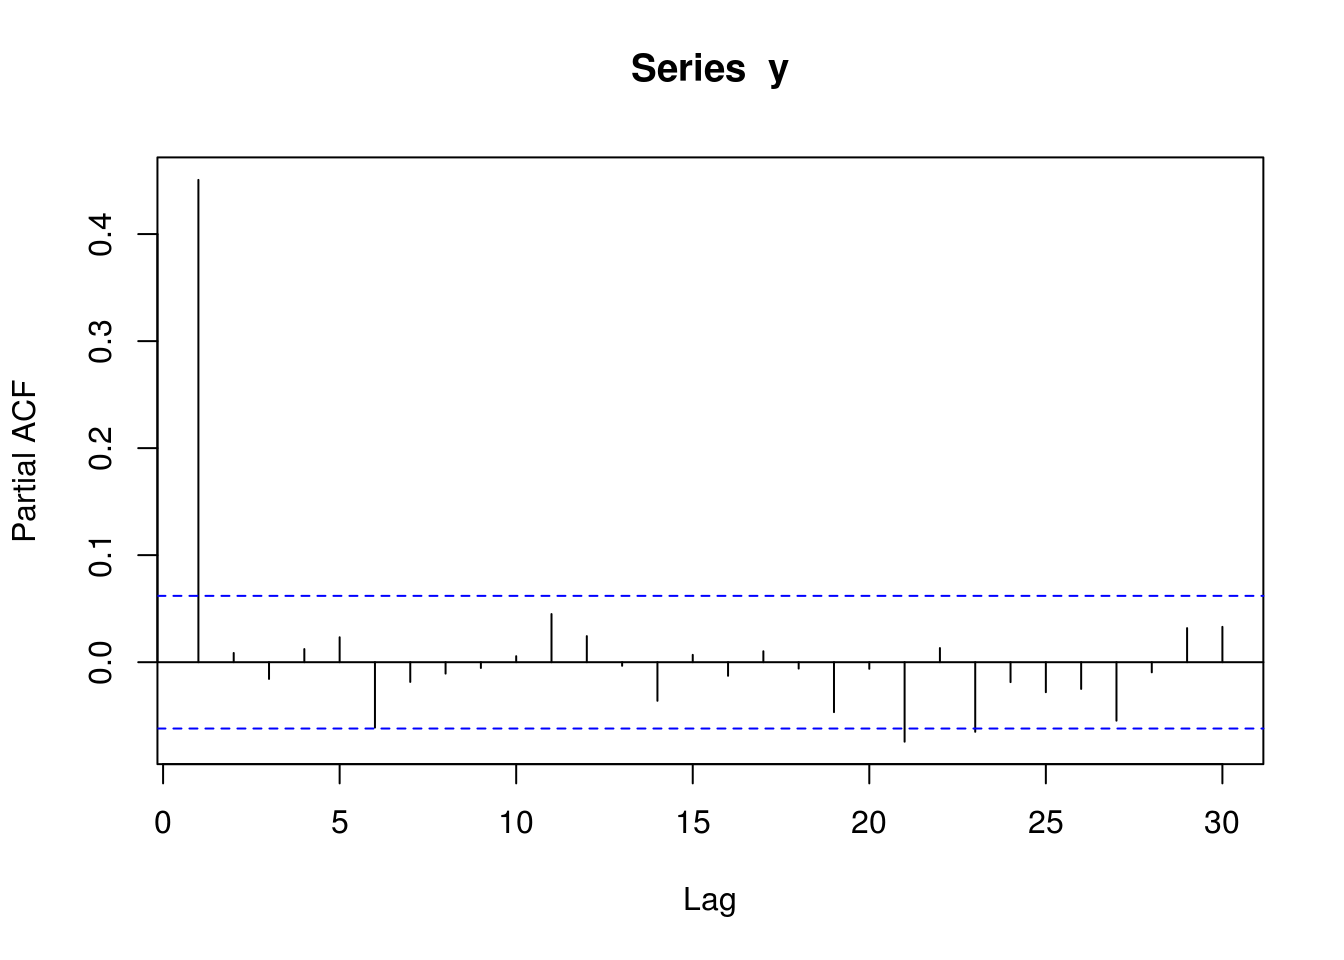
\includegraphics{website_files/figure-latex/unnamed-chunk-7-1.pdf}

\newpage

With \texttt{autoregressive} data, an \texttt{acf} plot contains a
number of decreasing lines. The following \texttt{acf} plot represents
some sort of \texttt{AR} data. Note that the \texttt{acf} plot displays
\texttt{lag\ 0} (which is pointless and can be ignored), while the
\texttt{pacf} plot does not.

\begin{Shaded}
\begin{Highlighting}[]
\KeywordTok{acf}\NormalTok{(y)}
\end{Highlighting}
\end{Shaded}

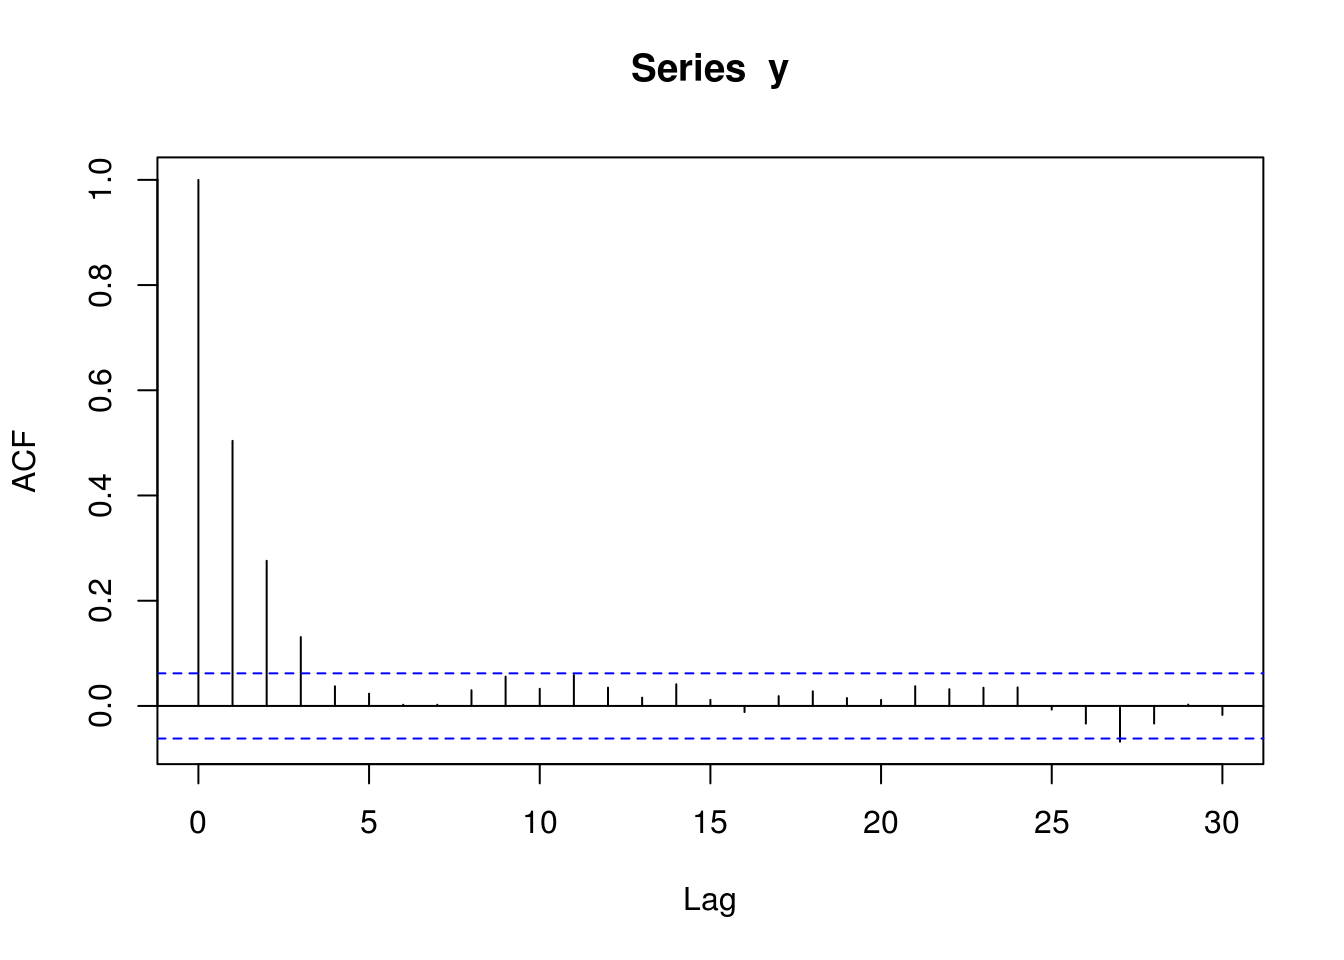
\includegraphics{website_files/figure-latex/unnamed-chunk-8-1.pdf}

\newpage 

\subsection{AR(2) data}\label{ar2-data}

\begin{Shaded}
\begin{Highlighting}[]
\NormalTok{y <-}\StringTok{ }\KeywordTok{round}\NormalTok{(}\KeywordTok{as.numeric}\NormalTok{(}\KeywordTok{arima.sim}\NormalTok{(}\DataTypeTok{model=}\KeywordTok{list}\NormalTok{(}\StringTok{"ar"}\NormalTok{=}\KeywordTok{c}\NormalTok{(}\FloatTok{0.5}\NormalTok{,}\FloatTok{0.4}\NormalTok{)), }\DataTypeTok{rand.gen =}\NormalTok{ rnorm, }\DataTypeTok{n=}\DecValTok{1000}\NormalTok{)))}
\end{Highlighting}
\end{Shaded}

The following \texttt{pacf} plot represents \texttt{AR(2)} data. This
means that each observation is correlated with its two preceeding
observations (\texttt{AR(2)}).

\begin{Shaded}
\begin{Highlighting}[]
\KeywordTok{pacf}\NormalTok{(y)}
\end{Highlighting}
\end{Shaded}

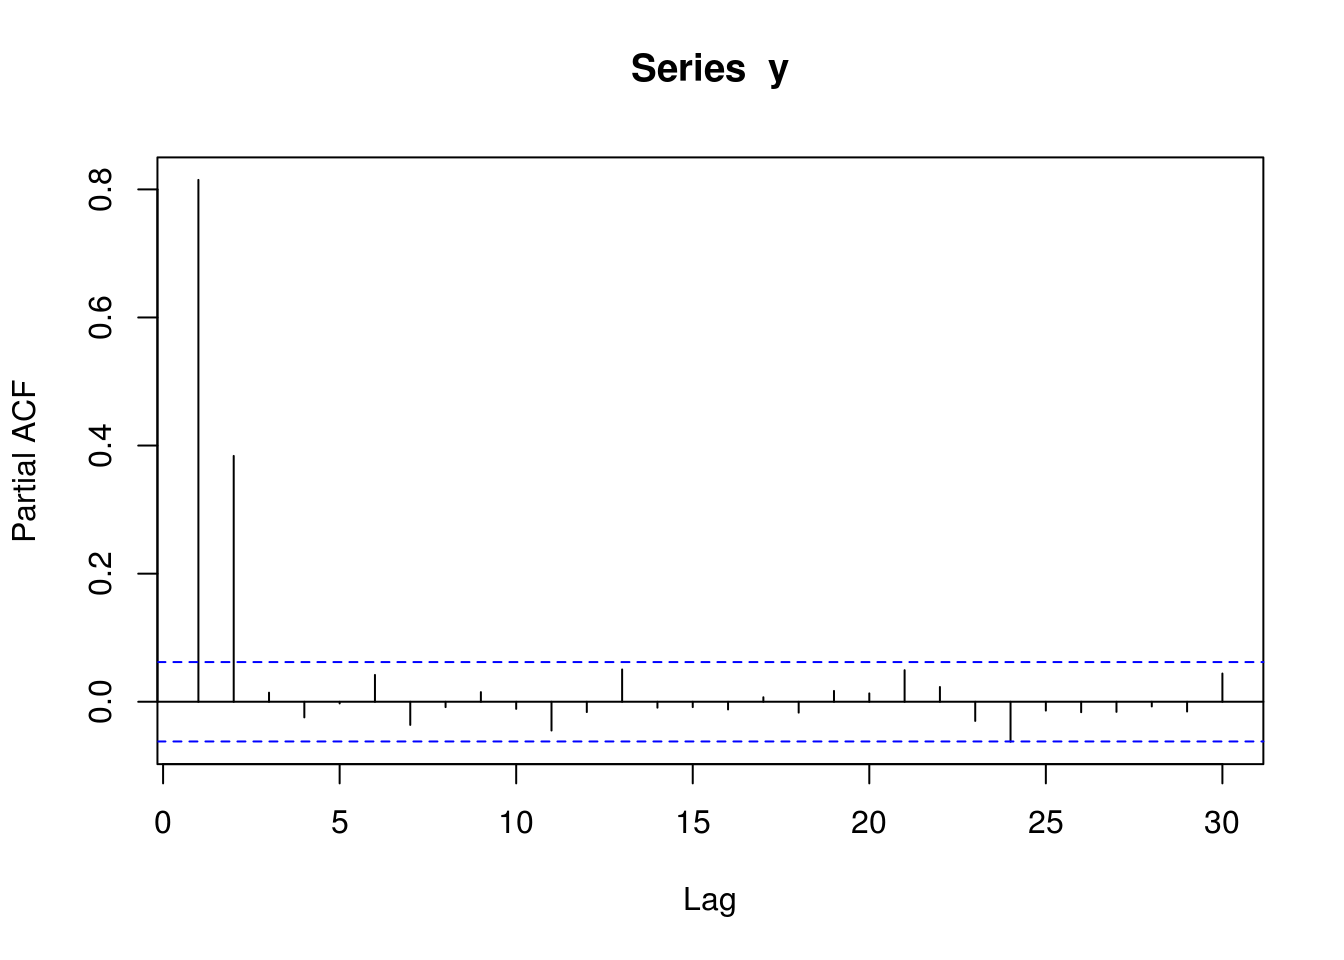
\includegraphics{website_files/figure-latex/unnamed-chunk-10-1.pdf}

\newpage

The following \texttt{acf} plot represents some sort of \texttt{AR}
data:

\begin{Shaded}
\begin{Highlighting}[]
\KeywordTok{acf}\NormalTok{(y)}
\end{Highlighting}
\end{Shaded}

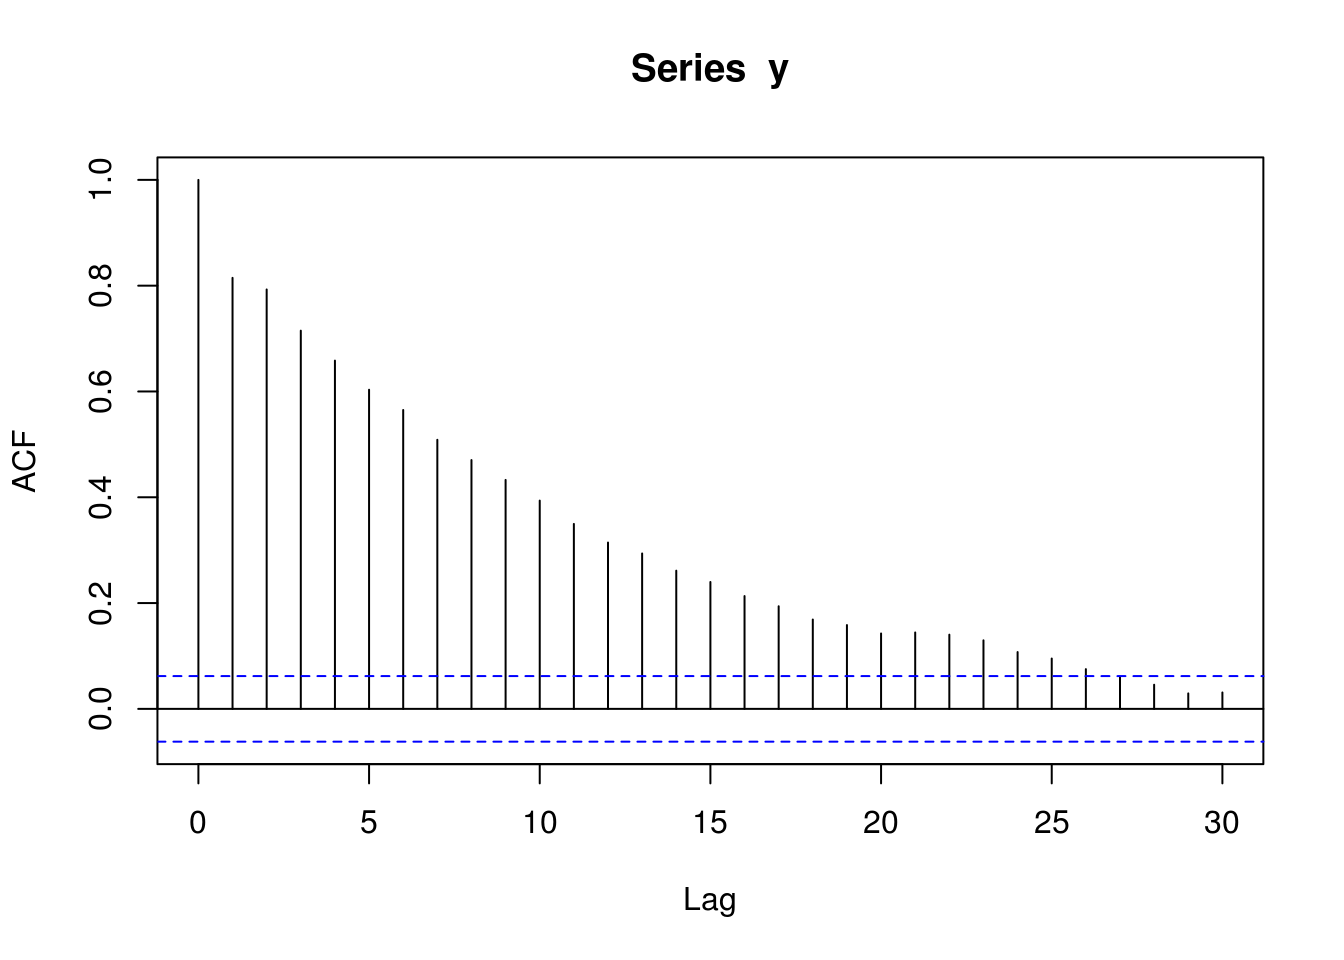
\includegraphics{website_files/figure-latex/unnamed-chunk-11-1.pdf}

\newpage 

\subsection{MA(1) data}\label{ma1-data}

\begin{Shaded}
\begin{Highlighting}[]
\NormalTok{y <-}\StringTok{ }\KeywordTok{round}\NormalTok{(}\KeywordTok{as.numeric}\NormalTok{(}\KeywordTok{arima.sim}\NormalTok{(}\DataTypeTok{model=}\KeywordTok{list}\NormalTok{(}\StringTok{"ma"}\NormalTok{=}\KeywordTok{c}\NormalTok{(}\FloatTok{0.9}\NormalTok{)), }\DataTypeTok{rand.gen =}\NormalTok{ rnorm, }\DataTypeTok{n=}\DecValTok{1000}\NormalTok{)))}
\end{Highlighting}
\end{Shaded}

With \texttt{moving\ average} data, a \texttt{pacf} plot contains a
number of decreasing lines. The following \texttt{pacf} plot represents
some sort of \texttt{MA} data.:

\begin{Shaded}
\begin{Highlighting}[]
\KeywordTok{pacf}\NormalTok{(y)}
\end{Highlighting}
\end{Shaded}

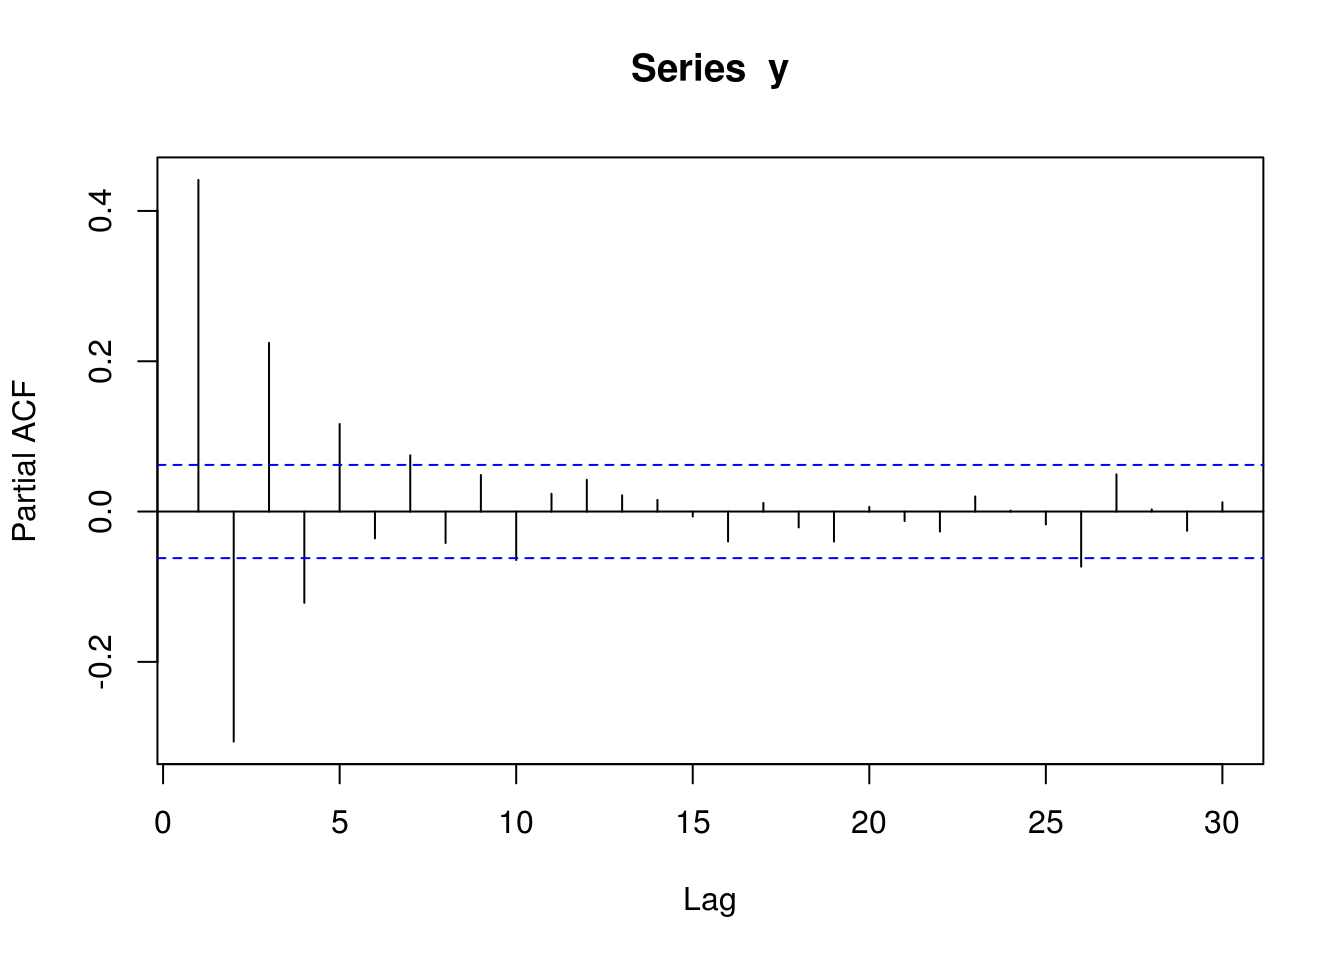
\includegraphics{website_files/figure-latex/unnamed-chunk-13-1.pdf}

\newpage

With \texttt{moving\ average} data, an \texttt{acf} plot contains a
number of sharp significant lines, demarking how many subsequent
observations have autocorrelation. i.e.~if one line is significant, it
means that each observation is only correlated with its preceeding
observation. If two lines are significant, it means that each
observation is correlated with its two preceeding observations. The
following plot represents \texttt{MA(1)} data. Note that the
\texttt{acf} plot displays \texttt{lag\ 0} (which is pointless and can
be ignored), while the \texttt{pacf} plot does not.

\begin{Shaded}
\begin{Highlighting}[]
\KeywordTok{acf}\NormalTok{(y)}
\end{Highlighting}
\end{Shaded}

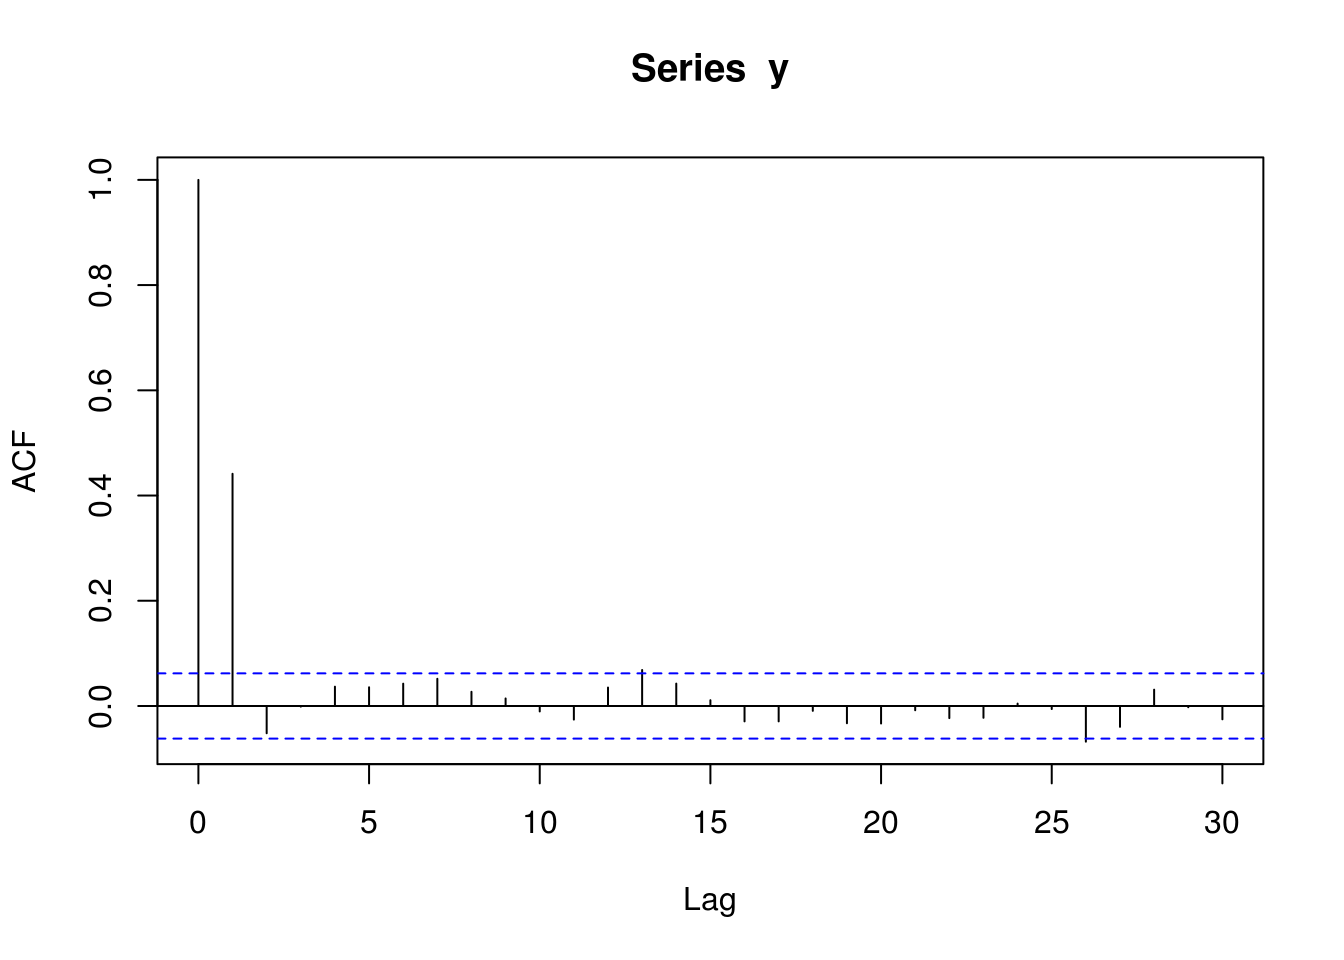
\includegraphics{website_files/figure-latex/unnamed-chunk-14-1.pdf}

\newpage 

\subsection{MA(2) data}\label{ma2-data}

\begin{Shaded}
\begin{Highlighting}[]
\NormalTok{y <-}\StringTok{ }\KeywordTok{round}\NormalTok{(}\KeywordTok{as.numeric}\NormalTok{(}\KeywordTok{arima.sim}\NormalTok{(}\DataTypeTok{model=}\KeywordTok{list}\NormalTok{(}\StringTok{"ma"}\NormalTok{=}\KeywordTok{c}\NormalTok{(}\FloatTok{0.9}\NormalTok{,}\FloatTok{0.6}\NormalTok{)), }\DataTypeTok{rand.gen =}\NormalTok{ rnorm, }\DataTypeTok{n=}\DecValTok{1000}\NormalTok{)))}
\end{Highlighting}
\end{Shaded}

The following \texttt{pacf} plot represents some sort of \texttt{MA}
data.

\begin{Shaded}
\begin{Highlighting}[]
\KeywordTok{pacf}\NormalTok{(y)}
\end{Highlighting}
\end{Shaded}

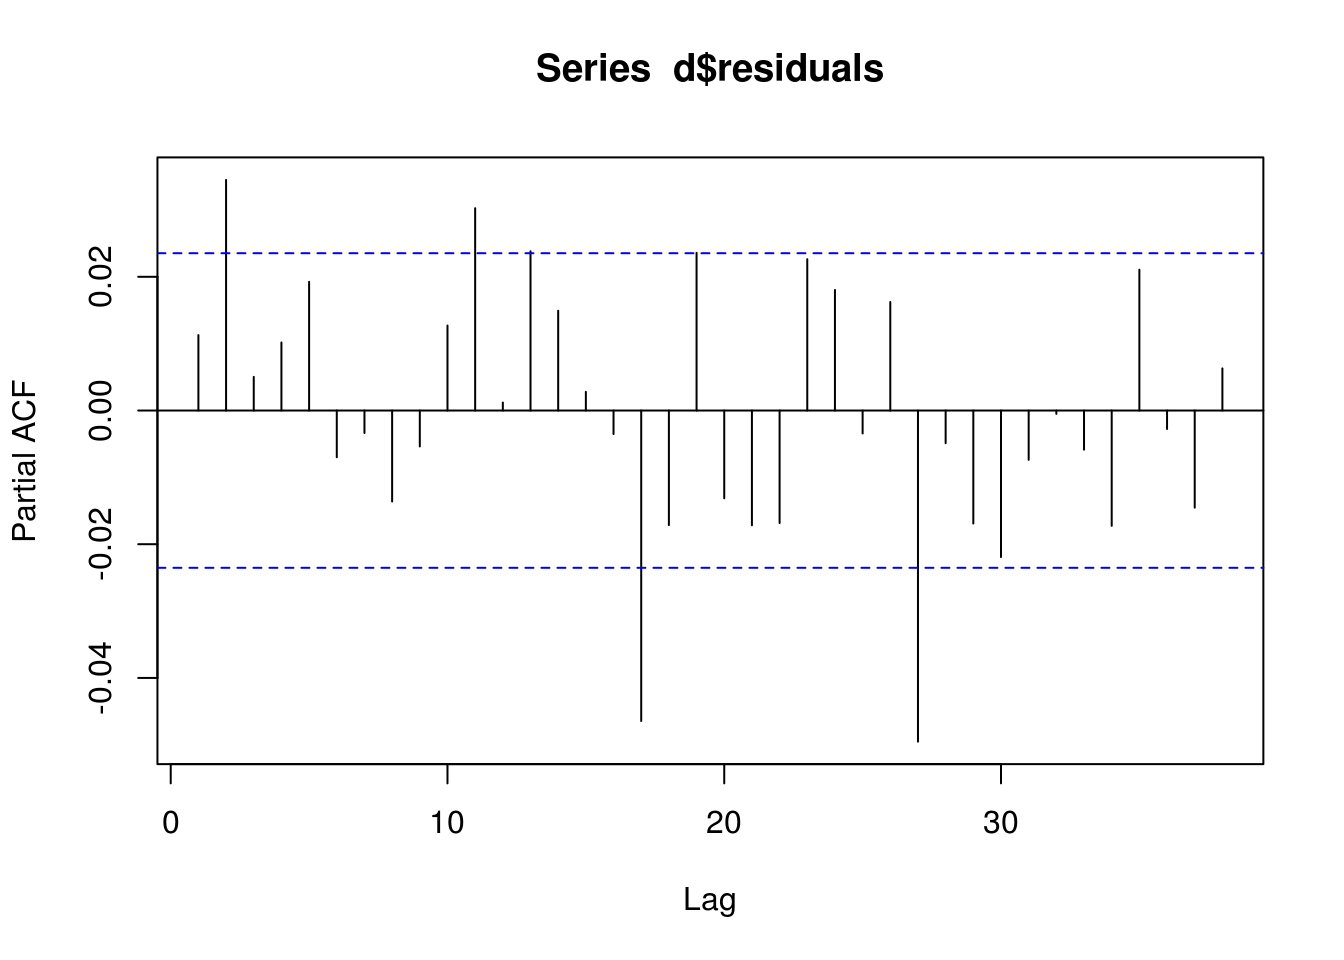
\includegraphics{website_files/figure-latex/unnamed-chunk-16-1.pdf}

\newpage

The following \texttt{acf} plot represents \texttt{MA(2)} data. This
means that each observation is correlated with its two preceeding
observations.

\begin{Shaded}
\begin{Highlighting}[]
\KeywordTok{acf}\NormalTok{(y)}
\end{Highlighting}
\end{Shaded}

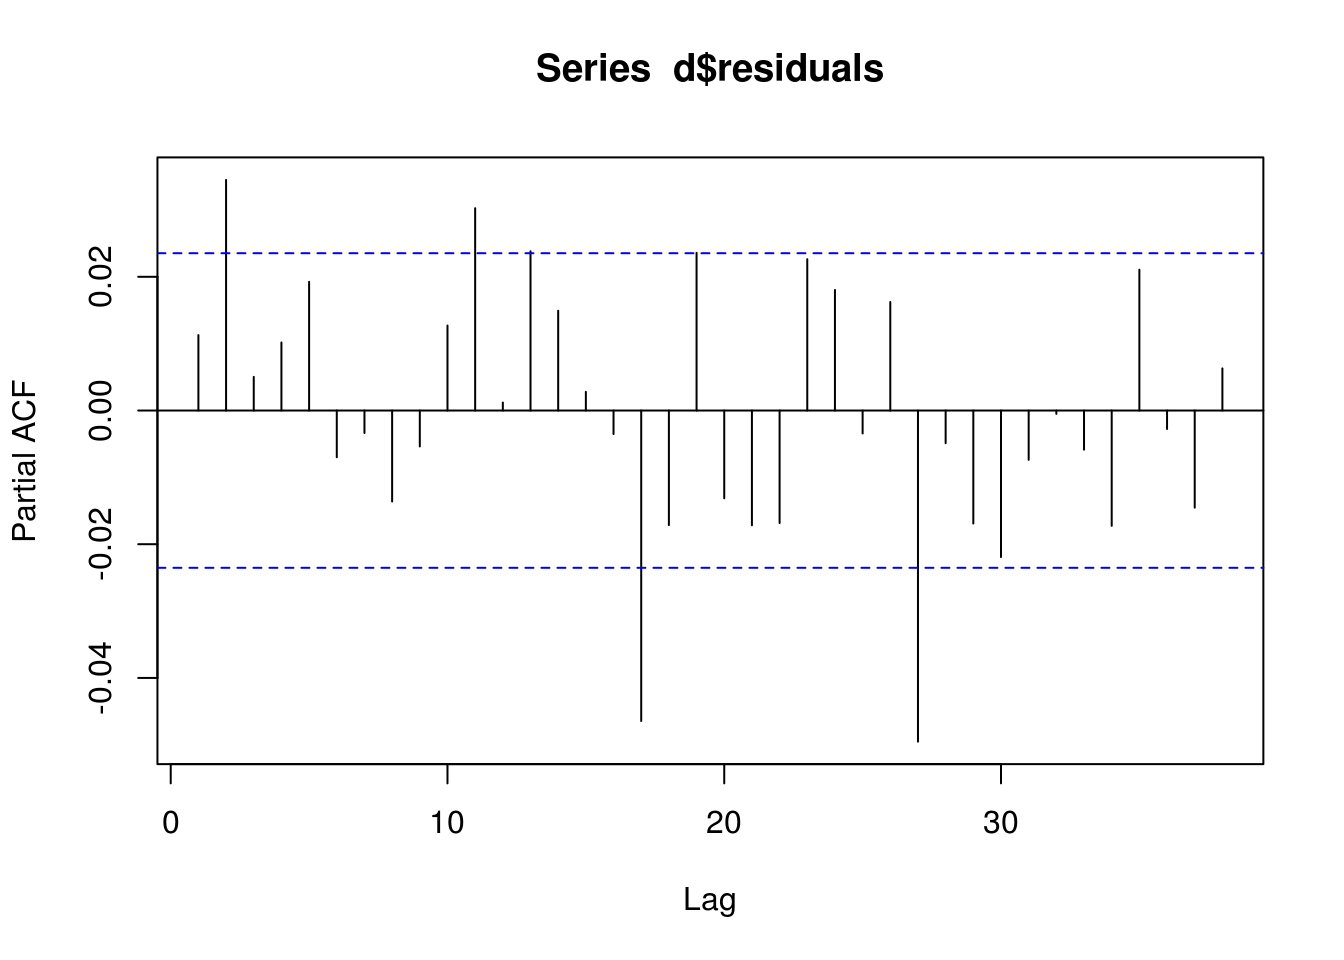
\includegraphics{website_files/figure-latex/unnamed-chunk-17-1.pdf}

\bibliography{book.bib,packages.bib}


\end{document}
